\documentclass[]{article}
\usepackage[spanish]{babel}
\usepackage{graphicx}
\usepackage[utf8]{inputenc}
\usepackage{fancyhdr}
\usepackage{lastpage}

\pagestyle{fancy}
\fancyhf{}
\rfoot{Page \thepage\hspace{1pt} de~\pageref{LastPage}}

\title{Practica 6}
\author{Guillermo Lopez Garcia}
\begin{document}

\maketitle

\textbf{Ejercicio 4.}
Como se puede apreciar, la mejor solución (la que ofrece mayor speed up) en este tipo de problemas,
donde es prioritario el cálculo numerico, es la solución concurrente de hilo grueso. En este solución,
es donde obtenemos mayor speed up, llegando incluso a tener speed up hiperlineal. \\

Esto es así debido a que nuestra maquina tiene un nivel de cache especial para trabajar con matrices
con instrucciones especiales del hardware en la microarquitectura de nuestro procesador. \\

No obstante, para la imagen pequeña que tratamos, la división del problema con hilo fino ofrece mejores
resultados que la solución secuencial (speed up = 1), pero obviamente a crear tantas tareas o hebras,
penalizamos en tiempo, ya que, al tener tantas hebras para tan pocos hilos lógicos (8 en el caso concreto de
mi máquina) implica cambios de contexto en nuestro sistema de una hebra a otra a la hora de ser atendida
por el procesador. \\

\begin{figure}
\centering
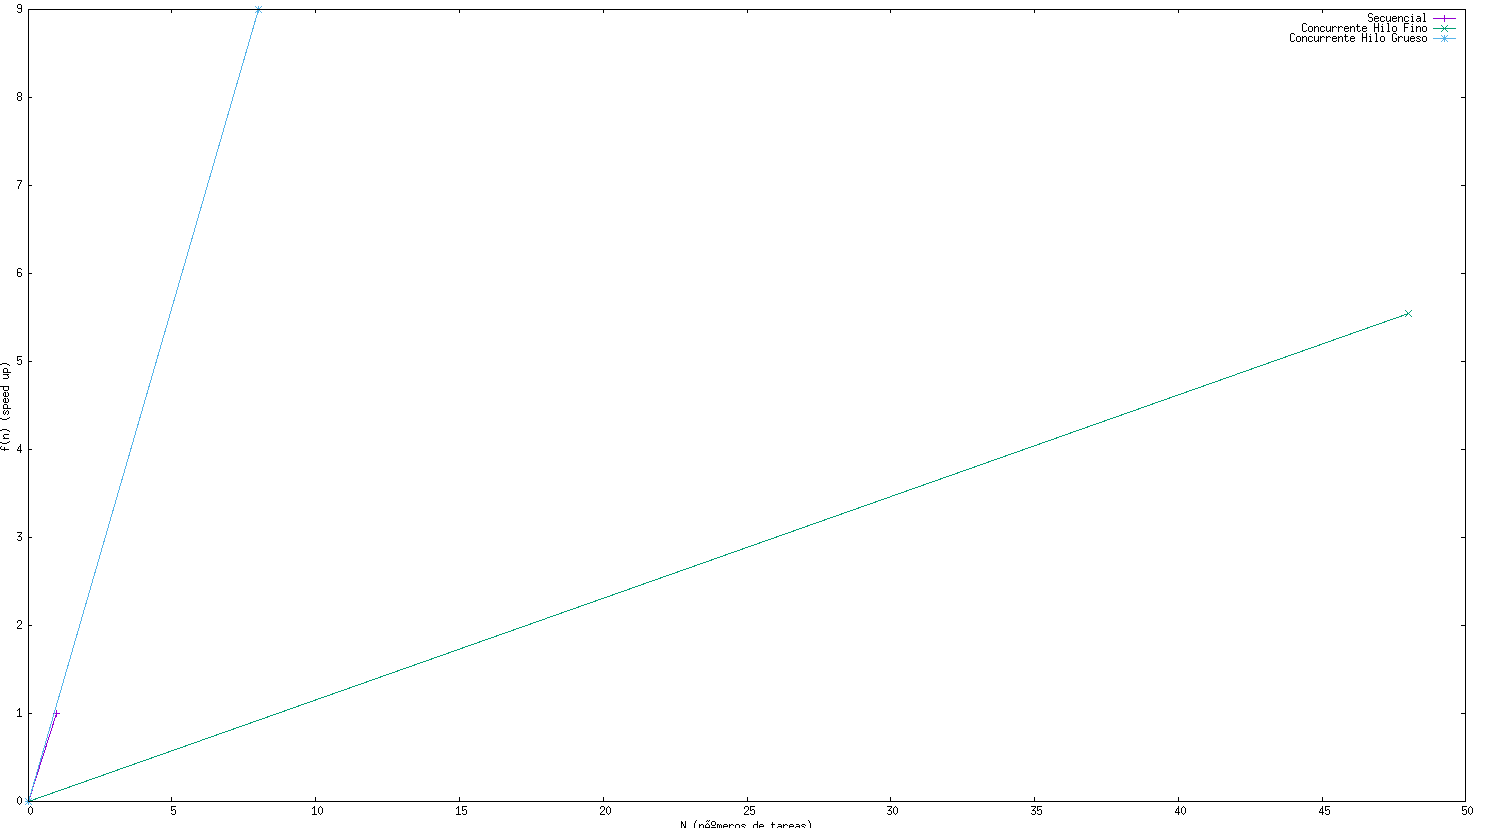
\includegraphics[width=\linewidth]{img.png}
\caption{Comparativa de Speed Up y Nº Hebras.}
\label{fig:comp}
\end{figure}

Por último aclarar que, claramente, la versión secuencial arroja un speed up igual a 1. No haría falta
ponerlo, ya que, el tiempo de la resolución de un problema secuencial respecto a su propia versión
secuencial siempre es igual. Por tanto, el speed up es igual a 1.

\end{document}
